\documentclass[aps,prd,twocolumn,amsmath,amssymb,floatfix,nofootinbib,10pt]{revtex4}
%\documentclass[aps,prd,amsmath,amssymb,floatfix,nofootinbib,12pt]{revtex4}

\usepackage{graphicx,epsfig}
\usepackage{amsmath,amssymb}
\usepackage{subfigure,epsfig}
%\usepackage{feynmp}
\usepackage{float}
%\DeclareGraphicsRule{.tif}{png}{.png}{`convert #1 `basename #1 .tif`.png}
%\DeclareGraphicsRule{.tif}{png}{.png}{`convert #1 `basename #1 .tif`.png}

\newcommand{\eg}{e.g.}
\newcommand{\Fermi}{\emph{Fermi}}
\newcommand{\VL}{Via Lactea}
\newcommand{\aquarius}{Aquarius}
\newcommand{\CDM}{CDM}
\newcommand{\LCDM}{\ensuremath{\Lambda}\CDM}
\newcommand{\NFW}{NFW}
\newcommand{\GNFW}{G\NFW}
\newcommand{\DM}{DM}
\newcommand{\SM}{SM}
\newcommand{\OM}{OM}
\newcommand{\mpl}{\ensuremath{m_{\mathrm{Pl}}}}
\newcommand{\somm}{\ensuremath{S}}
\newcommand{\mdm}{\ensuremath{m_{\chi}}}
\newcommand{\mv}{\ensuremath{m_{\phi}}}
\newcommand{\dd}{\mathrm{d}}
\newcommand{\Eqnname}{Equation}
\newcommand{\eqnname}{equation}
\newcommand{\Ngamma}{\ensuremath{N_{\gamma}}}
\newcommand{\Ngammai}{\ensuremath{N_{\gamma,i}}}
\newcommand{\Eth}{\ensuremath{E_{\mathrm{th}}}}
\newcommand{\sigmaannv}{\ensuremath{\langle\sigma v\rangle}}
\newcommand{\los}{los}
\newcommand{\order}{\ensuremath{\mathcal{O}}}
\newcommand{\sigv}{\ensuremath{\sigma_v}}
\newcommand{\lum}{\ensuremath{\mathcal{L}}}
\newcommand{\lumsmooth}{\ensuremath{\lum_{\mbox{{\footnotesize sm}}}}}
\newcommand{\lumsmoothc}{\ensuremath{\lum_{\mbox{{\footnotesize sm}},v=c}}}
\newcommand{\lumsmoothtoo}{\ensuremath{\overline{\mathcal{L}}}}
\newcommand{\lumsub}{\ensuremath{\lum_{\mbox{{\footnotesize sub}}}}}
\newcommand{\boost}{\ensuremath{B}}
\newcommand{\redr}{\ensuremath{\tilde{r}}}
\newcommand{\rhos}{\ensuremath{\rho_s}}
\newcommand{\rs}{\ensuremath{r_s}}
\newcommand{\dist}{\ensuremath{D}}
\newcommand{\norm}{\ensuremath{\mathcal{N}}}
\newcommand{\normnfw}{\ensuremath{\norm_1}}
\newcommand{\normeinasto}{\ensuremath{\norm_2}}
\newcommand{\rhominustwo}{\ensuremath{\rho_{-2}}}
\newcommand{\rminustwo}{\ensuremath{r_{-2}}}
\newcommand{\sommboost}{\ensuremath{\mathcal{S}}}
\newcommand{\clumpboost}{\ensuremath{\mathcal{C}}}
\newcommand{\alphaEinasto}{\ensuremath{\alpha}}
\newcommand{\Msol}{\ensuremath{M_{\odot}}}
\newcommand{\Mvir}{\ensuremath{M_{\mbox{{\footnotesize vir}}}}}
\newcommand{\Rvir}{\ensuremath{r_{\mbox{{\footnotesize vir}}}}}
\newcommand{\conc}{\ensuremath{c}}
\newcommand{\rhoc}{\ensuremath{\rho_{\mbox{{\footnotesize c}}}}}
\newcommand{\omegam}{\ensuremath{\Omega_{m}}}
\newcommand{\vcirc}{\ensuremath{v_{\mbox{{\footnotesize c}}}}}
\newcommand{\vmax}{\ensuremath{v_{\mbox{{\footnotesize max}}}}}
\newcommand{\rmax}{\ensuremath{r_{\mbox{{\footnotesize max}}}}}

%Journals
\newcommand{\aap}{Astron.~Astrophys.}
\renewcommand{\nat}{Nature}
\newcommand{\jhep}{J.~High.~Energy.~Phys.}
\newcommand{\astropartphys}{Astropart.~Phys.}
\newcommand{\mnras}{Mon.~Not.~Roy.~Astron.~Soc.}
\newcommand{\apjs}{Astrophys.~J.~Suppl.}
\newcommand{\apjl}{\apj}
\newcommand{\aj}{Astron.~J.}
\newcommand{\jcap}{J.~Cosmol.~Astropart.~Phys.}

\begin{document}

\title{Substructure Boosts to Dark Matter Annihilation from Sommerfeld Enhancement}
\author{Jo Bovy} \affiliation{Center for
Cosmology and Particle Physics, Department of Physics\\ New York
University, New York, NY 10003}

\date{\today}

\begin{abstract}
We discuss the implications of the Sommerfeld enhancement of the dark
matter annihilation cross section for the detection of dark matter
annihilation from subhalos in the Galactic halo. A robust prediction
of \CDM\ is that the Galactic halo is teeming with cold substructure,
and that the subhalos themselves contain even smaller substructure,
leading to an approximately self-similar distribution of substructure
all the way down to earth-mass halos. In addition to the boost to the
dark matter annihilation cross section from the high densities of
these subhalos, an additional boost due to Sommerfeld enhancement
results from the fact that they are kinematically cold. We take
subhalos from the large numerical $N$-body simulation \VL\ to study
the expected distribution of dark matter annihilation signals from
subhalos at a Sun-like position in a large dark matter halo hosting a
late-type galaxy. We also study the expected Sommerfeld enhanced
annihilation signal for the smallest, most-dark-matter-dominated, and
kinematically coldest dwarf spheroidal satellite galaxy Segue
1. Finally, we discuss the prospects for detecting annihilation
signals from microhalos.
\end{abstract}

%\keywords{}
\maketitle

\section{Introduction}

First two paragraphs straight from my paper with Glennys:

In the standard flat, Gaussian, adiabatic, and scale-invariant \LCDM\
paradigm $\sim\!80$ \% of the matter density of the Universe is in the
form of dark matter (\DM) \cite{2008arXiv0803.0547K}. The properties
of dark matter are largely unconstrained, although a weakly
interacting massive particle (WIMP) with a mass $\sim\!100$ GeV -- 1
TeV has many attractive features, including that it leads to a relic
density of dark matter that is remarkably close to the measured value
\cite{1996PhR...267..195J}. No interaction of dark matter either with
itself or with standard model (\SM) particles other than gravity has
ever been observed. However, at the present day we cannot exclude that
the dark sector is brimming with a rich phenomenology at
weak-interaction scales or lower.

One exciting possibility is that dark matter self-annihilates at a
level observable in the Galactic halo today. Detecting this
self-annihilation seems unlikely considering the standard
self-annihilation cross section --- $\sigmaannv_{\mathrm{ann}}
\lesssim 3 \times 10^{-26} $ cm$^3$ s$^{-1}$ for consistency with the
observed relic density. However, there are various mechanisms to boost
the annihilation signal to a value larger by a few orders of
magnitude, e.g., clumpiness of the dark halo
\cite{1993ApJ...411..439S,1999PhRvD..59d3506B,2008A&A...479..427L,2008ApJ...686..262K}
or a combination of coannihilations and Sommerfeld enhancement
\cite{2005PhRvD..72j3521P,2008arXiv0812.0360L}. The possibility of
detecting the \DM\ annihilation signal has attracted much attention
recently because of the anomalous excesses of high energy electrons
and positrons reported by two different experimental groups: the
Payload for Antimatter Exploration and Light-nuclei Astrophysics
(PAMELA) satellite, which saw a sharp upturn in the positron fraction
$e^+/(e^++e^-)$ from 10 -- 100 GeV \cite{Adriani:2008zr}, and the
Advanced Thin Ionization Calorimeter (ATIC) group, which reported an
excess in the combined number of electrons and positrons at energies
500 -- 800 GeV \cite{2008Natur.456..362C}. The PAMELA result on the
positron fraction confirms earlier results
\cite{1969ApJ...158..771F,1975ApJ...199..669B,1987ApJ...312..183M,1994ApJ...436..769G,Barwick:1997ig,Beatty:2004cy,Aguilar:2007yf}
and can be explained by \DM\ annihilation
\cite{2002PhLB..536..263K,2004PhRvD..69j3509H,2008arXiv0810.5344C}. There
is still a good chance that these anomalies can be obviated by
conventional astrophysical effects, e.g., pulsars
\cite{1995A&A...294L..41A,2008arXiv0810.1527H,2008arXiv0810.2784Y,2008arXiv0812.4457P}. Nevertheless,
a plethora of models has been proposed in the last few months
explaining the PAMELA and ATIC results in terms of \DM\ annihilation
into electron-positron pairs (e.g.,
\cite{2008arXiv0810.5557H,ArkaniHamed:2008qn,2008arXiv0811.0399F,2008arXiv0811.1555I,2008arXiv0811.3357C,2008arXiv0811.3641C,2008arXiv0812.2196A}),
a description which also naturally accounts for other experimental
anomalies, such as the ``WMAP haze''
\cite{Finkbeiner:2003im,Dobler:2007wv,Hooper:2007kb}, EGRET
observations of an excess of high-energy gamma-rays in the Galactic
center \cite{Strong:2005zx}, and recent HESS measurements of the flux
of very high-energy electrons \cite{2008arXiv0811.3894H}. Model
building is complicated by the fact that PAMELA did not observe a
similar excess in the ratio of anti-protons to protons
\cite{2008arXiv0810.4994A}, which means that the coupling of the \DM\
particles to quarks must somehow be suppressed.


Of course, the largest obstacle currently to modeling the PAMELA/ATIC
signal with \DM\ annihilation is the very large boost factors ($10^4$
-- $10^5$) with respect to the fiducial $\langle \sigma v
\rangle_{\mathrm{ann}} \approx 3 \times 10^{-26} $ cm$^3$ s$^{-1}$
needed to lead to an observable annihilation flux. The boost factors
from the clumpiness of the dark matter halo is expected to be small
\cite{2008A&A...479..427L,2008Natur.454..735D,2008ApJ...686..262K,2008Natur.456...73S},
typically of the order 1 -- 10. Therefore, a different mechanism must
be reponsible for the large boosts necessary. One such mechanism that
has received much attention lately is the Sommerfeld enhancement
\cite{sommerfeld31a,2003PhRvD..67g5014H,2004PhRvL..92c1303H,2005PhRvD..71f3528H,2005PhRvD..71a5007H,2006PhRvD..73e5004H,2008NuPhB.800..204C,2008JHEP...07..058M,2008arXiv0812.0559M,2008arXiv0812.0360L}. The
Sommerfeld enhancement is a generic effect present whenever there is
an attractive force acting between the dark matter particles, \eg, due
to a Yukawa interaction or a gauge interaction through vector bosons
\cite{ArkaniHamed:2008qn}. The main effect of this attractive force is
to enhance the annihilation cross section with a factor proportional
to $\beta^{-1}$ ($\beta \equiv v/c$), this is known as ``$1/v$''
enhancement. There are regions in the parameter space made up of the
dark matter mass \mdm, the force carrier mass \mv, and the force
``fine-structure constant'' $\alpha \equiv$ coupling$^2$/$4 \pi$ in
which the enhancement is near a resonance, where it approximately
behaves as $\beta^{-2}$. However, the enhancement levels off at a
certain $\beta$ due to the finite range of the attractive force ---
large ($\alpha \sim\!10^{-1}$ -- $10^{-3}$) attractive forces with
infinite range lead to a burst of \DM\ annihilation in the first \DM\
halos formed at $z$ $\sim$ 100 -- 200 which would lead to observable
effects incompatible with measurements of the diffuse extragalactic
gamma-ray background today and the cosmic microwave background
\cite{2008arXiv0810.3233K}.



BOVY: Say something here about clumpiness of the halo: much more than
the following: \cite{1998MNRAS.300..146G,johnston98a,2003MNRAS.339..834H,2008ApJ...688..277T,2002MNRAS.330..778W,2002MNRAS.330..792K,koposov,Koposov:2009ru}



\section{The Sommerfeld enhancement}

The simplest example of the Sommerfeld effect that contains all of the
generic features described in the introduction is that of the
Sommerfeld enhancement due to an attractive Yukawa type force mediated
by a spin-0 boson $\phi$ between the \DM\ particles, and we adopt that
description here. The Sommerfeld effect is a non-perturbative effect
in the sense that in the language of quantum field theory it comes
about from Feynman diagrams in which the force carrier is exchanged
many times before the annihilation actually happens, giving rise to so
called ``ladder diagrams''. However, we can study the Sommerfeld
effect in simple, non-relativistic quantum mechanics (see the appendix
in Ref.~\cite{ArkaniHamed:2008qn}). We are instructed to solve the
radial Schr{\"o}dinger equation (in natural units)
\begin{equation}\label{eq:sommdiff1}
\frac{1}{\mdm} \frac{\dd^2 \psi(r)}{\dd r^2} + \frac{\alpha}{r}e^{-\mv r} \psi(r) = -\mdm \beta^2 \psi(r)\, ,
\end{equation}
subject to the boundary condition $\dd\psi/\dd r = i \mdm \beta \psi$
as $r \rightarrow \infty$. Here $\mdm$ and $\mv$ are the mass of the
dark matter and the force carrier, respectively. Using the
substitution $r \rightarrow \alpha \mdm r$ this becomes
\begin{equation}\label{eq:sommdiff2}
\frac{\dd^2 \psi(r)}{\dd r^2} + \frac{1}{r}e^{-\mv r/(\alpha \mdm)} \psi(r) = -\frac{\beta^2}{\alpha^2} \psi(r)\, ,
\end{equation}
with boundary condition
\begin{equation}
\psi \propto e^{i\beta r/\alpha} \qquad \mbox{ as } r \rightarrow\infty\, .
\end{equation}
The Sommerfeld enhancement \somm\ is then given by
\begin{equation}
\somm = \frac{|\psi(\infty)|^2}{|\psi(0)|^2}\, .
\end{equation}
From \eqnname\ (\ref{eq:sommdiff2}) it can be seen that the Sommerfeld
enhancement is only a function of two variables, which can be chosen
as $\alpha/\beta$ and $\alpha \mdm/\mv$. The qualitative features of
\eqnname\ (\ref{eq:sommdiff2}) have been widely discussed before and
are easily derived, and, therefore, we will merely mention them here
without proof (see, \eg,
Refs.~\cite{ArkaniHamed:2008qn,2008arXiv0812.0360L}). When the kinetic
energy of the collision is much larger than the product of the force
carrier mass and the coupling, then the Yukawa interaction can be
approximated as an attractive Coulomb interaction, for which an
analytical solution in terms of hypergeometric functions exists. The
Sommerfeld enhancement is simply given by
\begin{equation}
\somm = \frac{\pi \alpha}{\beta} (1 - e^{-\pi\alpha/\beta})^{-1}\, .
\end{equation}
From this we see why the Sommerfeld enhancement is often referred to
as a ``$1/v$'' enhancement for small velocities $\beta \ll 1$. In the
limit of a vanishing interaction ($\alpha/\beta \ll 1$) the Sommerfeld
enhancement disappears as $\somm \rightarrow 1$. The $1/v$ behavior,
which diverges for small $\beta$ and leads to an overproduction of
high-energy photons in the early Universe \cite{2008arXiv0810.3233K},
levels off due to the finite range of the Yukawa interaction at a
velocity $\beta \approx \mv/\mdm$ and settles on a value $\somm \approx
\alpha \mdm/\mv$. However, at some parameter combinations the Yukawa
potential has bound states, at which there are large boosts to the
annihilation cross section which go approximately as $\somm \propto
\beta^{-2}$. These resonance regions, however, are cut-off at small
$\beta$ due to the finite lifetime of the bound state. We expect these
three different behaviors ($1/v$, saturation at low $v$, and resonance
effects due to the existence of bound states) to be generic among
different models of the Sommerfeld enhancement (see also the
discussion in the appendix of Ref.~\cite{ArkaniHamed:2008qn}).

\Eqnname\ (\ref{eq:sommdiff2}) can also be numerically integrated
efficiently, by integrating the solution $\psi(r) = e^{i\beta
r/\alpha}$ inwards from a radius satisfying
\begin{equation}
\frac{1}{r}e^{-\mv r/(\alpha \mdm)} \ll \frac{\beta^2}{\alpha^2} \, .
\end{equation}
In the Coulomb regime ($\mdm \beta^2 \gg \alpha \mv$) this means that
the starting value should be such that $r \gg \alpha^2/\beta^2$;
otherwise we should start at $r \gg \alpha \mdm/\mv$. Figure
\ref{fig:sommb34} shows the Sommerfeld enhancement in the parameter plane
made up off $\alpha$ and $\mv/\mdm$. All of the qualitative features
we discussed above are present: In the Coulomb regime (lower part of
the two panels) we see that the enhancement scales as $\alpha$,
leveling off at $\somm \approx 1$ when $\alpha$ becomes small; The
fact that the upper left corner of both panels is approximately the
same shows that the Sommerfeld enhancement saturates at $\beta \approx
\mv/\mdm$; The sharp diagonal lines in the upper right of both panels
is the resonance region, in which the enhancement is sharply
peaked. Because of the scaling properties of \eqnname\
(\ref{eq:sommdiff2}) shifting $\log\beta$ is equivalent to shifting
both $\log\alpha$ and $\log \mv/\mdm$ by the same amount. Therefore,
the $\beta$ behavior of the enhancement can also be read off from
these figures along diagonals. Inspection of the resonance diagonals
in the second panel of Figure \ref{fig:sommb34} shows that the enhancement
grows as $\beta^{-2}$ in these regions.



\begin{figure}[t]
\centering
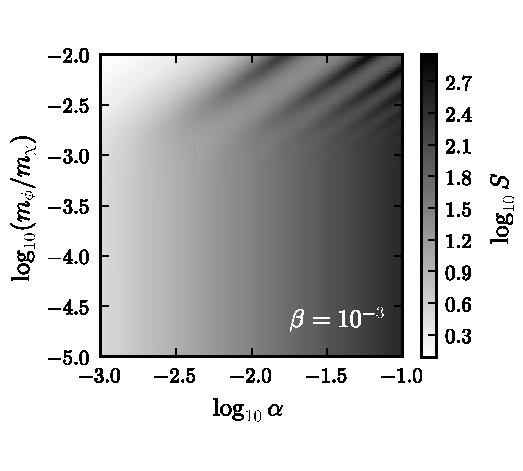
\includegraphics{2d-3.eps}
\\
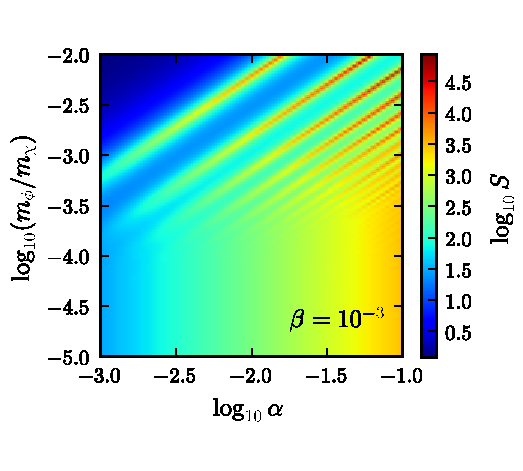
\includegraphics{2d-4.eps}
\caption{Sommerfeld enhancement as a function of the particle physics
parameters for two different values of the relative velocity
$\beta$. Because of the scaling properties of \eqnname\
(\ref{eq:sommdiff2}) the behavior of the Sommerfeld enhancement as a
function of $\log_{10}\beta$ can actually be read off along diagonals
in the plane.}%\
\label{fig:sommb34}%
\end{figure}



Of course, when considering the Sommerfeld enhancement of a halo of a
certain velocity dispersion $\sigv$ we need to average the Sommerfeld
enhancement over the velocity distribution of that halo. We will
approximate the velocity distribution of the halo as a single Gaussian
distribution with velocity dispersion $\sigv$, in which case we need
to average the enhancement over a truncated Maxwell-Boltzmann
distribution
\begin{equation}\label{eq:maxboltz}
f(v) \propto \left\{
\begin{array}{rl}
v^2\, e^{-v^2/2\sigv^2}  & \qquad v \leq v_{\mathrm{esc}}\\
0 & \qquad v > v_{\mathrm{esc}}\, ,\\
\end{array} \right.
\end{equation}
in which we set the escape velocity to $v_{\mathrm{esc}} =
\sqrt{2}\,\sigv$. Note that in the pure $1/v$ regime this averaging
will tend to sustain the $1/v$ behavior up to a factor $\order(1)$,
since then
\begin{equation}
\int_0^\infty \dd v \, v^2\, e^{-v^2/2\sigv^2}
\somm\left/\int_0^\infty \dd v \, v^2\, e^{-v^2/2\sigv^2} \right.\propto
\frac{1}{\sigv}\, ,
\end{equation}
since the truncation does not significantly influence the
result. Similarly, in the resonance region the $1/v^2$ behavior is
conserved by the averaging. When the enhancement has leveled off the
averaging has no effect.



\begin{figure*}[t]
\includegraphics[clip=]{avg-3_64.eps}%%BoundingBox: 178 291 400 474
\includegraphics[clip=]{avg-4_128.eps}\\%%BoundingBox: 190 291 418 474
\includegraphics[clip=]{avg-5_128.eps}%%BoundingBox: 178 291 400 474
\includegraphics[clip=]{avg-6_128.eps}%%BoundingBox: 190 291 418 474
\caption{Sommerfeld enhancement factor as a function of the particle
physics parameters averaged over a Maxwell-Boltzman velocity
distribution with velocity dispersion \sigv\ for four different orders
of magnitude of the velocity dispersion (all velocities are relative
to the speed of light).}%
\label{fig:sommavg}%
\end{figure*}




\section{Substructure boosts from Sommerfeld enhancement}
The photon flux from \DM\ annihilation from a solid angle
$\Delta\Omega$ along a given line-of-sight (\los) is given by
\begin{equation}\label{eq:flux}
\begin{split}
\frac{\dd \Ngamma}{\dd A \,\dd t}  = &
\int_{\Eth}^{\mdm}\dd E\, \sum_i \frac{\dd
\Ngammai}{\dd E} \,\frac{\sigmaannv_i}{\mdm^2}\,
\somm\left(\mv/\mdm,\alpha,\sigv\right)\,\\
& \times \int_{\Delta\Omega}\,\frac{\dd\Omega}{4\pi}\,\int_{\mathrm{\los}} \dd l\,
\rho^2(l)\, .
\end{split}
\end{equation}
In this \Eth\ is the treshold energy of the detector, $i$ denotes
(possibly) different final states of the \DM\ annihilation, $\frac{\dd
\Ngammai}{\dd E}$ is the spectrum from the annihilation to that state,
$\sigmaannv_i$ is the annihilation cross section to state $i$ (without
the Sommerfeld enhancement), $\somm\left(\mv/\mdm,\alpha,\beta\right)$
is the Sommerfeld enhancement which we have factored out of the cross
section, and $\rho(l)$ is the \DM\ density along the line-of-sight. We
emphasize that this framework also allows us to consider different
final annihilation products, such as the electrons and positrons
supposedly seen by PAMELA/ATIC.


We will focus our analysis on the quantity on the ``structure quantity''
\lum($M$), which we define here as
\begin{equation}\label{eq:structquant}
\lum(M)\equiv\somm\left(\mv/\mdm,\alpha,\sigv\right)\,\int_{\Delta\Omega}\,\frac{\dd\Omega}{4\pi}\int_{\mathrm{\los}}
\dd l\, \rho^2(l)
\end{equation}
This structure quantity does not only depend on the mass and internal
properties of the \DM\ halos in which we are interest, it depends on
the particle physics parameters as well. We will keep all of the other
factors in \eqnname\ (\ref{eq:flux}) fixed. However, in order to
derive actual numbers for the photon flux from \DM\ annihilation, we
briefly describe the other quantities appearing in \eqnname\
(\ref{eq:flux}) here.

\subsection{Some details of the particle physics that do not particularly concern us here}


For the annihilation cross section without taking account of any
Sommerfeld enhancement we will adopt the fiducial value $\sigmaannv =
3 \times 10^{-26} $ cm$^3$ s$^{-1}$. The energy spectrum of the \DM\
annihilation depends on the model used to describe the \DM\ and its
interactions and it is outside of the scope of this paper to provide a
detailed treatment of this for different \DM\ models. Therefore, we
use an annihilation spectrum appropriate for neutralino dark matter,
which provides a reasonable fit to a variety of different annihilation
products. Since the energy spectrum contributes a multiplicative
factor to the \DM\ annihilation flux, the effect of different
annihilation spectra can be incorporated by simply multiplying our
results with the appropriate factor. The neutralino dark matter
annihilation spectrum we use has the form
\cite{1998APh.....9..137B,2004PhRvD..70j3529F}
\begin{equation}\label{eq:annspectrum}
\frac{\dd \Ngamma}{\dd E} = \frac{a_1}{\mdm} \left(\frac{E}{\mdm}\right)^{-3/2}\, \exp\left[-a_2\frac{E}{\mdm}\right]\, ,
\end{equation}
with parameters $a_1\sim 1$ and $a_2 \sim 10$, depending on the
details of the annihilation process
\cite{2004PhRvD..70j3529F}. Integrating this spectrum using a
threshold energy appropriate for \Fermi\, $\Eth = 4$ GeV, and choosing
a \DM\ mass, $\mdm = 700$ GeV, we find that
\begin{equation}
\int_{\Eth}^{\mdm}\dd E\, \sum_i \frac{\dd
\Ngammai}{\dd E} \approx 17\, ,
\end{equation}
with any differences due to variations in $(a_1,a_2)$ and $\mdm$
between different models leading to changes of a factor $\order(10)$. 




\subsection{The Dark Matter profile}


The density profile of dark matter halos has been discussed
extensively in the last few years. While the shape of the outer
density profile seems to have converged in the various numerical
simulations of \DM\ halos and a consensus has been reached, the
detailed shape of the inner density profile is still a hot topic of
debate. The main point of contention is whether the density profile is
cusped near the center of the \DM\ halo, and if so, how steep this
cusp is, or whether the density stays finite near the center. Since
this discussion has a non-negligible impact on the prospects for \DM\
annihilation detection, we will briefly discuss the various plausible
density profiles.

The inner structure of \DM\ halos is one of the key predictions of the
\CDM\ paradigm, and over a decade ago it was shown that the
spherically averaged density profiles of \DM\ halos are well described
by a universal profile, the so-called \NFW\ profile
\cite{1995MNRAS.275..720N,1996ApJ...462..563N,1997ApJ...490..493N},
depending only on the virial mass of the halo and its
concentration. Moreover, the concentration was shown to depend
systematically on the halo mass
\cite{1996ApJ...462..563N,1997ApJ...490..493N,2001MNRAS.321..559B,2001ApJ...554..114E,2007MNRAS.381.1450N,2008MNRAS.387..536G}. This
profile was found to provide a good fit to many numerical simulations
(\eg,
\cite{1996MNRAS.281..716C,1997MNRAS.286..865T,1997ApJS..111...73K}).
While there seems to be a consensus between different numerical
simulations on the shape of the outer density profile, no agreement
was reached on the inner density structure of the \DM\ halos found in
the simulations. The \NFW\ profile has an inner slope of -1, other
studies, however, found evidence for steeper inner slopes
\cite{1997ApJ...477L...9F,1998ApJ...499L...5M,1999MNRAS.310.1147M,2000ApJ...544..616G,2001ApJ...554..903K,2001ApJ...557..533F,2004MNRAS.353..624D},
shallower inner slopes \cite{1998ApJ...502...48K}, or didn't find any
convergence toward a power-law behavior
\cite{2003MNRAS.338...14P}. Even the universality of the density
profile was brought into question
\cite{2000ApJ...529L..69J,2000ApJ...535...30J}.

More recently, high-resolution numerical simulations have essentially
ruled out the steepest cusps, such as Moore's profile, which has an
inner cusp with logarithmic slope of -1.5, however steeper inner cusps
than the original \NFW\ profile are still observed in numerical
simulations \cite{2005MNRAS.364..665D}. Other recent simulations find
inner slopes that are shallower than an \NFW\ profile
\cite{2008MNRAS.385..545K,2008arXiv0808.2981S,2008arXiv0810.1522N},
although there is a growing consensus that the logarithmic slope of
the inner density profile is a quantity that hasn't fully converged
yet in any numerical simulation. It also has become apparent in recent
years that the inner density profile of \DM\ halos might not be
described by a power-law divergence, but that, on the contrary, the
logarithmic slope becomes ever shallower, leading to a cored density
profile
\cite{2004MNRAS.349.1039N,2005ApJ...624L..85M,2006AJ....132.2685M,2006AJ....132.2701G,2006MNRAS.365..147S,2008arXiv0808.2981S,2008MNRAS.391.1685S,2008arXiv0810.1522N}. Therefore,
density profiles such as the Einasto profile
\cite{einasto65a,1989A&A...223...89E} have been shown to provide an
excellent fit to the numerical simulations with the highest resolution
yet \cite{2008MNRAS.391.1685S,2008arXiv0808.2981S}.

Since the photon flux from \DM\ annihilations depends on the density
squared of the \DM\, the exact form of the inner density profile has
important ramifications for the detectability of \DM\
annihilation. This has been widely discussed before in the context of
various \DM\ annihilation models (\eg,
\cite{1998APh.....9..137B,1999PhRvL..83.1719G,2000PhRvD..62l3005C,2000PhLB..494..181G,2002PhRvD..66b3509T,2002PhRvD..66l3502U,2003MNRAS.339..505T,2004ApJ...601...47A,2008JCAP...07..013B,2008arXiv0811.3744B,2008arXiv0812.3895B}). Roughly
speaking, the annihilation flux is smaller for inner density profiles
which are cored, and larger for inner density profiles which show a
cuspy behavior. The steeper the slope of the inner cusp, the larger
the \DM\ annihilation flux (for obvious reasons). Since the core
vs.~cusp debate is still undecided we will consider \DM\ distribution
models of both types.

The cuspy \DM\ profile we will use is a generalized \NFW\ profile (\GNFW):
\begin{equation}\label{eq:NFW}
\rho(r) = \frac{\rhos}{\redr^\gamma\left(1+\redr\right)^{3-\gamma}};\qquad \redr = r/\rs\, ,
\end{equation}
in which \rhos\ is a characteristic density and \rs\ a characteristic
(scale-)radius.  The original \NFW\ profile is recovered for $\gamma$
= 1 \cite{1997ApJ...490..493N}, which we will use as the fiducial
cuspy model in what follows. Varying the value of the inner
logarithmic slope $\gamma$ will allow us to describe the effect of
steeper and shallower inner slopes than the \NFW\ model. Note that
this functional form does \emph{not} include the exact form of Moore's
profile; this need not concern us since inner cusps as steep as
Moore's profile have been as good as excluded by the latest numerical
simulations.

The contribution of the \DM\ density profile on the structure quantity
\lum\ can be simply evaluated in the context of any density model. As
in Ref.~\cite{2007PhRvD..75h3526S} we assume that the distance
\dist\ is much larger than the scale-radius of the \DM\ halo. For an
\NFW\ profile 90\% of the flux originates from the region with one
scale-radius, and we will, conservatively, only take contributions to
the \DM\ annihilation flux coming rom this region for all the
\GNFW\ profiles. Therefore, we find that 
\begin{equation}\label{eq:lumrhosrsNFW}
\int_{\Delta\Omega}\,\frac{\dd\Omega}{4\pi}\,\int_{\mathrm{\los}} \dd
l\, \rho^2(l)= \normnfw(\gamma)\, \frac{\rhos^2\, \rs^3}{\dist^2}\, .
\end{equation}
The normalization of this relationship depends on the logarithmic
slope of the inner cusp and is given by
\begin{equation}\label{eq:normgammaNFW}
\normnfw(x) = 4 \pi  \, \frac{2^{2x-5}\left(-16+11x-2x^2\right)}{-30+47x-24x^2+4x^3}\, .
\end{equation}
The normalization for the \NFW\ profile is $7\pi/6$ and it depends
strongly on the value of the logarithmic slope of the inner density
profile, as can be seen in Figure \ref{fig:normgammaNFW}. The lower
panel of Fig.~\ref{fig:normgammaNFW} shows the fraction of the \DM\
annihilation flux coming from region within one scale-radius of the
halo. For reasonable values of the inner slope this fraction is in the
range 80 -- 95\%.

\begin{figure}[t]
\centering
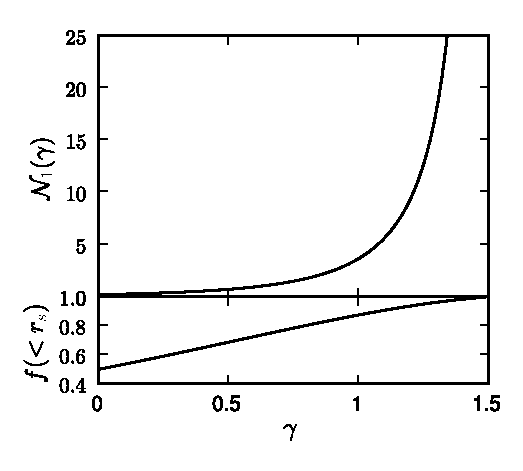
\includegraphics{normgammaNFW.eps}
\caption{Top: Normalization of the $\lum \propto \rhos^2\,
\rs^3/\dist^2$ relation of \eqnname\ (\ref{eq:lumrhosrsNFW}) for the
\GNFW\ profile. The functional dependence of the normalization on the
exponent $\gamma$ in the profile given in \eqnname\ (\ref{eq:NFW}) is
given in \eqnname\ (\ref{eq:normgammaNFW}). Bottom: Fraction of the
emission that comes from the region within \rs.}%\
\label{fig:normgammaNFW}%
\end{figure}

The Einasto profile is characterized by an ever-decreasing logarithmic
inner slope. It's functional dependence on the radius is given by
\begin{equation}\label{eq:einasto}
\rho (r) = \rhominustwo\, \exp\left[-\frac{2}{\alpha}\left\{\left(\frac{r}{\rminustwo}\right)^{\alpha}-1\right\}\right]\, .
\end{equation}
Here, \rhominustwo\ is the density at the radius \rminustwo\ where the
local slope is -2 and \alphaEinasto\ is a parameter often fixed at a
value $\sim\!0.17$ \cite{2008MNRAS.391.1685S}. As above, assuming
$\dist \gg \rminustwo$, calculating the flux originating from within
the radius \rminustwo, we find that
\begin{equation}\label{eq:lumrhosrsEinasto}
\int_{\Delta\Omega}\,\frac{\dd\Omega}{4\pi}\,\int_{\mathrm{\los}} \dd
l\, \rho^2(l)= \normeinasto(\alpha)\, \frac{\rhominustwo^2\, \rminustwo^3}{\dist^2}\, .
\end{equation}
The normalization depends on the value of \alphaEinasto\ and is given
by
\begin{equation}\label{eq:normgammaEinasto}
\normeinasto(x) = 4 \pi \, 2^{-6/\alpha}\,e^{4/\alpha}\,
\alpha^{-1+3/\alpha}\,
\gamma\left[\frac{3}{\alpha},\frac{4}{\alpha}\right]\,
,
\end{equation}
where $\gamma[a,z]$ is the lower incomplete gamma function. The
dependence of this normalization on \alphaEinasto\ is shown in Figure
\ref{fig:normgammaEinasto}. In order to compare the Einasto profile as
described here, we can relate the parameters $(\rhos,\rs)$ of the
profile in \eqnname\ (\ref{eq:NFW}) to the parameters
$(\rhominustwo,\rminustwo)$ of the Einasto model by calculating the
radius at which the logarithmic slope of the density versus radius
profile equals -2. Thus, we find that
\begin{equation}
\rminustwo = \rs,  \qquad \qquad \rhominustwo = \frac{\rhos}{2^{3-\gamma}}\, .
\end{equation}

Note that the \DM\ annihilation flux from the Einasto profile,
although it seems larger from Figs.~\ref{fig:normgammaNFW} and
\ref{fig:normgammaEinasto}, is actually smaller in general, since
there is a factor of 2$^{6-2\gamma}$ involved in going from one to the
other.

\begin{figure}[t]
\centering
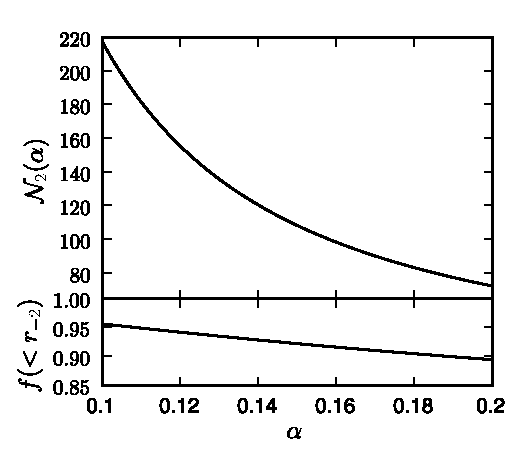
\includegraphics{normgammaEinasto.eps}
\caption{Top: Normalization of the $\lum \propto \rhominustwo^2\,
\rminustwo^3/\dist^2$ relation of \eqnname\
(\ref{eq:lumrhosrsEinasto}) for the Einasto profile. The functional
dependence of the normalization on $\alpha$ in the profile given in
\eqnname\ (\ref{eq:einasto}) is given in \eqnname\
(\ref{eq:normgammaEinasto}). Bottom: Fraction of the emission that
comes from the region within \rminustwo.}%\
\label{fig:normgammaEinasto}%
\end{figure}

Further on it will sometimes be useful to describe the \DM\ density
profiles by different parameters than a characteristic density and
radius. Another set of parameters is given by a concentration
parameter and a mass. The concentration for both the \GNFW\ profile as
for the Einasto profile is given by
\begin{equation}\label{eq:concdef}
\conc \equiv \frac{\Rvir}{\rminustwo}\, .
\end{equation}
A characteristic mass is given by the virial mass \Mvir. The virial
mass of the \GNFW\ profile is given by
\begin{equation}\label{eq:Mvirdef}
\Mvir = 4\pi\rhos\rs^3 \left[ - (-\conc)^\gamma\,\conc^{-\gamma} B(-c;3-\gamma,\gamma-2)\right]\, ,
\end{equation}
in which $B(z;a,b)$ is the incomplete Beta function, given by the
familiar form $f(c) = \ln(1+c)-c/(1+c)$ in the special case of the
\NFW\ profile. The virial mass for the Einasto profile is given by
\begin{equation}
\Mvir = 4\pi\rhominustwo\rminustwo^3 \frac{1}{\alphaEinasto} \exp\left(\frac{3\ln \alphaEinasto + 2 - \ln 8}{\alphaEinasto}\right) \gamma\left[\frac{3}{\alphaEinasto},\frac{2}{\alphaEinasto}\conc^\alphaEinasto\right]\, .
\end{equation}
In this last expression $\gamma\left[a,z\right]$ is the lower
incomplete gamma function. The density can then be expressed in terms
of the concentration by using the definition of the virial mass:
$\Mvir \equiv 4\pi/3 \Delta \rhoc \Rvir^3$, where $\Delta = 178\,
\omegam^{0.45} \approx 100$
\cite{1996MNRAS.282..263E,1998ApJ...495...80B}, and \rhoc\ is the
critical density.

Another pair of parameters that one can use to characterize the \DM\
density profile is the maximum circular velocity \vmax\ and the radius
at which this maximum occurs, \rmax. These parameters are especially
well-suited when dealing with numerical simulations, since they can be
readily read off from the raw simulation data. The circular velocity
is given by
\begin{equation}
\vcirc^2(r) \equiv \frac{G M(r)}{r} = \vcirc^2(\Rvir)\frac{c}{f(c)}\frac{f(x)}{x}\, ,
\end{equation}
in which $x \equiv r/\rminustwo$ and $f(x)$ is given by
$B(-x;3-\gamma,\gamma-2)$ in the case of a \GNFW\ profile and by
$\gamma\left[\frac{3}{\alphaEinasto},\frac{2}{\alphaEinasto}x^\alphaEinasto\right]$
in the case of an Einasto profile. One can find \rmax\ by (numerically) solving the equation
\begin{equation}
\frac{\dd}{\dd x}\left[ \frac{f(x)}{x}\right] = 0\, ,
\end{equation}
and \vmax\ follows then immediatly.


\subsection{Calculating the total boost}

As is customary, we will write the total structure quantity \lum($M$) as a
sum of a smooth component and a substructure component:
\begin{equation}
\lum(M) = \lumsmooth(M) + \lumsub(M)\, .
\end{equation}
The smooth contribution to the structure quantity is the product of
the Sommerfeld enhancement \somm\ and the line-of-sight integral over
the \DM\ density squared, given for the different \DM\ density
profiles in \eqnname s (\ref{eq:lumrhosrsNFW}) and
(\ref{eq:lumrhosrsEinasto}). Therefore,
\begin{equation}
\lumsmooth(M) = \somm \, \lumsmoothc(M)\, ,
\end{equation}
in which \lumsmoothc\ is the luminosity that would come from the
smooth component of the halo in the absence of Sommerfeld
enhancememnt.

We can now write
\begin{equation}
\begin{split}
\lum(M) & = \somm\,\lumsmoothc(M) + \lumsub(M)\\
&= \left[ \somm + \frac{\lumsub(M)}{\lumsmoothc(M)}\right] \lumsmoothc(M)\, .
\end{split}
\end{equation}
We will from now on write the substructure boost as \boost(M). Then we
have the following
\begin{equation}\label{eq:boost}
\begin{split}
\boost(M) & \equiv \frac{\lumsub(M)}{\lumsmoothc(M)} = \frac{1}{\lumsmoothc(M)} \int \dd m \, \frac{\dd N}{\dd m} \lum(m)\\
&= \frac{1}{\lumsmoothc} \int \dd m\, \frac{\dd N}{\dd m} \left[ \somm(m) + \boost(m) \right] \lumsmoothc(m)\, .
\end{split}
\end{equation}
Here we have introduced the subhalo mass function $\dd N/\dd m$, which
gives the abundance of subhalos of mass $m$.

Before proceeding we should specify the upper and lower limits of the
integral appearing in \eqnname\ (\ref{eq:boost}). The integration over
ever smaller substructures is cut-off at the size of the smallest
subhalos. The mass scale at which this cut-off occurs is the thermal
free-streaming scale, a \DM\ model-dependent quantity, which in many
\DM\ models lies in the range 10$^{-6}$ -- 10$^{-12}$ \Msol
\cite{1999PhRvD..59d3517S,2001PhRvD..64h3507H,2004MNRAS.353L..23G,2005PhRvD..71j3520L,2006PhRvL..97c1301P}. The
upper limit to this integral is some fraction $q$ of the halo mass
$M$, since the abundance of substructure does not continue up to this
mass scale.

In order to calculate the total boost from substructure to the
annihilation cross section, we will write all of the quantities
appearing in \eqnname\ (\ref{eq:boost}) as a function of the mass
$m$. For instance, from numerical simulations, the subhalo mass
function is well constrained to follow a power-law type behavior:
\begin{equation}\label{eq:massfraction}
\frac{\dd N}{\dd \ln m}
\propto \left(\frac{m}{M}\right)^n\, .
\end{equation}
The value of the exponent $n$ is still under debate. The two highest
resolution $N$-body simulations yet, the \aquarius\ and \VL\
projects, both find values for $n$ that put roughly equal amounts of
mass per subhalo mass decade. While the \VL\ simulation seems to
prefer a value $n = -1$
\cite{2006ApJ...649....1D,2008ApJ...686..262K}, which would lead to a
logarithmically diverging total mass in substructures if the subhalo
abundance were not cut off at the thermal free-streaming limit of the
dark matter, the \aquarius\ project prefers a value $n = -0.9$
\cite{2008MNRAS.391.1685S}. As the \aquarius\ project has made
detailed convergence studies that support their claim for a value of
$n$ that is shallower than -1, we will adopt the value $n = -0.9$ as
our fiducial value, although even shallower slopes have also been
observed \cite{2002PhRvD..66f3502H}. The same slope has also been
observed in other simulations \cite{2004MNRAS.355..819G}.

With the exponent $n$ fixed, we turn to the normalization of the
relation given in \eqnname\ (\ref{eq:massfraction}). As one might
expect by now, different high-resolution numerical simulations give
different answers to this question as it relates to the abundance of
subhalos of Galactic subhalos. The problem of the normalization is
complicated by the fact that numerical simulations have only recently
begun to be able to resolve substructure in subhalos in a Galaxy-size
halo. While the simulations generally agree that the resolved
substructure abundance of subhalos in the host halo adds up to
$\sim\!10$\% of the total mass of the halo
\cite{1998MNRAS.300..146G,1999ApJ...522...82K,2004MNRAS.353..624D,2003ApJ...598...49Z,2007ApJ...657..262D,2007ApJ...667..859D},
the question of whether the substructure abundance in subhalos is just
a scaled-down version of the substructure abundance in the host halo
remains unresolved. One would not expect the abundance to be
self-similar, since, while substructure in both the main host halo and
subhalos gets diminished by tidal disruptions, substructure in the
subhalos does not get replenished by the infall of halos from the
field, as is the case for the host halo. Nevertheless, many numerical
simulations do find approximately self-similar substructure abundances
\cite{1999ApJ...524L..19M,2007ApJ...659.1082S}. Recently, the
\aquarius\ simulation has concluded from its simulation that the
substructure abundance is not self-similar, although the deviation
from the self-similar relation is small
\cite{2008MNRAS.391.1685S}. Therefore, we will adopt a normalization
here which places 10\% of the mass of the subhalo in the form of
``resolved'' substructure, where we adopt the definition that resolved
substructure is in halos of mass $\gtrsim 10^{-5} M$.

In the previous section we calculated $\lumsmoothc$ for the different
\DM\ density profiles and found in all cases that
\begin{equation}
\lumsmoothc(m) \equiv \lumsmoothc(\rho(m),r(m))\, ,
\end{equation}
for a characteristic density $\rho$ and radius $r$, the exact
definition of which depends on the specific \DM\ density profile
used. In order to find the mass dependence of $\lumsmoothc$, we use
the description of the \DM\ density profile in terms of virial mass
\Mvir\ and concentration \conc. We then make use of the fact that many
simulations have found a relation between the concentration of halos
and their mass
\cite{2001MNRAS.321..559B,2001ApJ...554..114E,2008MNRAS.387..536G,2007MNRAS.381.1450N},
such that everything depends only on the mass. This relation is well
established over a large range in halo masses, and we will adopt the
particular relationship found in Ref.~\cite{2007MNRAS.378...55M}
\begin{equation}\label{eq:concscaling}
\conc = 10.5 \, \left(\frac{\Mvir}{10^{12}\, \Msol}\right)^{-0.11}\, ,
\end{equation}
in good agreement with the results of other, similar analyses
\cite{2001MNRAS.321..559B,2005MNRAS.357..387K}, although the
normalization of the concentration-mass relation is about 15\% lower
than the original relation. However, the concentration of subhalos is
generally larger than the concentration of field halos of the same
mass as a result of tidal mass-loss
\cite{1998MNRAS.300..146G,2008ApJ...673..226P,2004MNRAS.355..794H,2005ApJ...635..931B,2004ApJ...608..663K}. This
is a small effect, of order 10\%, and we will investigate later
whether it significantly influences our results.

The only remaining quantity in \eqnname\ (\ref{eq:boost}) that we
haven't related to the mass of the subhalo yet, is the Sommerfeld
enhancement factor \somm. The Sommerfeld enhancement depends on the
mass of the subhalo through the velocity dispersion. Therefore, we
need to relate the velocity dispersion of a \DM\ subhalo to its
velocity dispersion. It is important to note that all we really need
is an approximate relationship between the velocity dispersion and the
halo mass which fits well the range of Galactic size halos to a scale
not much smaller than the mass scale of the smallest dwarf Spheroidals
known today, since in most cases the Sommerfeld enhancement will
saturate at velocity dispersions of the order of the velocity
dispersion of the dwarf Spheroidals.

On the scale of clusters there is a well-defined relationship between
the mass of a \DM\ halo and its one-dimensional velocity dispersion
which one can derive from adiabatic scaling arguments
\cite{1998ApJ...495...80B} given by
\begin{equation}\label{eq:vdispscaling}
\sigma \propto m^{1/3}\, .
\end{equation}
This scaling relation can be easily derived in the case of an
isothermal distribution function \cite{2008gady.book.....B}, since
then
\begin{equation}
\rho(r) = \frac{\sigma^2}{2\pi G r^2}\, ,
\end{equation}
from which \eqnname\ (\ref{eq:vdispscaling}) immediatly follows. This
scaling relation has been found to describe numerical simulations of
cluster-sized halos extremely well
\cite{1991ApJ...383...95E,1995MNRAS.275..720N,1995AJ....110...21C,1996ApJ...469..494E,1996MNRAS.281..716C,1998ApJ...495...80B}.From
recent numerical simulations it seems that we can use this relation
even for subhalos of subhalos in a Galaxy sized dark matter halo. In
Ref.~\cite{2008MNRAS.391.1685S} it is shown that the relation between
the maximum circular velocity of a subhalo and its mass is well fit by
a power-law of the type
\begin{equation}
m \propto \vmax^{3.5}\, .
\end{equation}
By a simple estimate of the velocity dispersion using the virial
theorem, we can use the maximum circular velocity as a measure of the
halos velocity dispersion. This would give $\sigv \propto
m^{1/3.5}$. Alternatively, we could use the circular velocity at the
virial radius as a measure of the velocity dispersion. In the case of
an \NFW\ profile we have that
\begin{equation}
\frac{\vmax^2}{\vcirc(\Rvir)^2} \propto \frac{c}{f(c)}\, ,
\end{equation}
in which $f(x) = \ln(1+c) - c/(1+c) \approx 2.6 (c/33)^{0.4}$ in the
relevant concentration range. Using \eqnname\ (\ref{eq:concscaling}),
this gives
\begin{equation}
\sigv \propto M^{0.32}\, .
\end{equation}
Therefore, we will use (as a rough approximation) the scaling relation
given in \eqnname\ (\ref{eq:vdispscaling}).


\section{A typical distribution of signals in a halo}


\section{Segue 1}


\section{Microhalos}


{\bf Acknowledgments:}
NASA 07-ADP07-0099.



\bibliographystyle{apsrev}
\bibliography{ann}




\end{document}
